% Springer Nature journal version, using the official sn-jnl class (December 2024 template package).
% Build: latexmk -pdf main.tex
% The reference style option (sn-mathphys-num) gives numbered references; change it to the style your target journal asks for.
% Fill every [bracketed] placeholder and check the target journal's Instructions for Authors before submission.
\documentclass[pdflatex,sn-mathphys-num]{sn-jnl}

\usepackage{graphicx}
\usepackage{amsmath,amssymb,amsfonts}
\usepackage{xcolor}
\usepackage{booktabs}
\usepackage{url}
\DeclareUrlCommand\burl{\urlstyle{rm}}

\raggedbottom

\begin{document}

\title[Spatial Gesture Control]{Spatial Gesture Control: Controlling a Laptop with Head Orientation and Smartwatch Pinch Gestures}

\author*[1]{\fnm{Vaibhav} \sur{Bisht}}\email{vaibhavbisht78@gmail.com}

\affil*[1]{\orgdiv{[Department]}, \orgname{[Institution]}, \orgaddress{\city{[City]}, \country{[Country]}}}

\abstract{We present and evaluate a system that lets a person control a laptop without touching it. The user looks at a calibrated screen location, pinches to grab a virtual volume knob, turns the wrist to change the volume and pinches again to release. Head orientation comes from consumer Sony headphones. Wrist motion and raw photoplethysmography (PPG) come from a Samsung Galaxy Watch over Bluetooth Low Energy, and all inference runs on the laptop behind a fail-closed safety chain. Because the watch cannot see the fingers, we recorded wrist signals with camera hand landmarks as reference timing annotations. We evaluated detectors as continuous event detectors, counting caught pinches against false activations per hour of no-gesture time. Wrist PPG alone generalised poorly to a new day (AUC 0.60--0.64), and six robustness methods did not change this. Fusing the inertial sensors raised worst-split AUC from 0.789 to 0.837, and firing at the score's peak added 4--12 recall points. A three-network 1-D convolutional model on nine raw channels outperformed tree ensembles, but held-out days varied widely (43\% of 372 starts pooled; about two thirds on the newer days). A later model trained on hand-corrected labels caught 47 of 57 pinch-in starts with no false activations over 0.48~h on its development evaluation set (median latency 442~ms), a result we reproduced by replaying the stored model. Median-based normalisation removed a motion-induced blind spot. We report the system design, data pipeline and results, and analyse the evaluation and labelling practices that determined whether offline results predicted live behaviour.}

\keywords{Gesture recognition, Smartwatch, Photoplethysmography, Inertial sensing, Head tracking, Wearable computing, Event detection}

\maketitle

% Shared body of the JOURNAL version. Included by main.tex in the IEEE journal and Springer Nature versions.
% Declarations and back matter live in each main.tex, because their form differs by publisher.

\section{Introduction}\label{sec:intro}

Laptops are still controlled through a keyboard, a pointer or a touch surface, although many people now wear sensors on the head and the wrist for most of the day. Noise-cancelling headphones contain motion sensors that report where the head points, and a smartwatch measures wrist motion and the optical blood-volume signal known as photoplethysmography (PPG). This article asks whether these everyday wearables can replace the keyboard for a simple spatial control: a virtual volume knob that the user looks at, grabs with a finger pinch, turns with the wrist and releases with a second pinch.

The interaction is easy to describe and hard to build. A watch cannot see the fingers, so a pinch must be inferred indirectly from changes in PPG and from small motions of the wrist. Everyday activity such as typing, reaching or scratching produces similar signals, and both signals change between days and strap fits. Three devices with independent clocks take part, and the output changes a real operating-system setting, so a wrong decision must never escalate.

We designed, built and evaluated such a system between 27 July and 7 November 2026, and we report both the engineering and the research that led to a working detector. We address three research questions:
\begin{itemize}
  \item \textbf{RQ1.} Can raw wrist PPG from a stock smartwatch detect the start of a pinch in continuous use, across days?
  \item \textbf{RQ2.} How much do the watch's inertial sensors, the trigger rule and the model family change detection performance?
  \item \textbf{RQ3.} Which evaluation and labelling practices are needed so that offline results predict live behaviour?
\end{itemize}

Our contributions are:
\begin{itemize}
  \item A cross-platform desktop coordinator that fuses Sony headset orientation with Samsung Galaxy Watch motion and raw PPG and drives system volume through a recipe engine with a fail-closed safety chain (Section~\ref{sec:system}).
  \item A data pipeline that records watch signals with camera hand landmarks as reference timing annotations, keeps hand corrections separate from the original labels, aligns three clocks and trains one binary detector per gesture label (Sections~\ref{sec:data} and~\ref{sec:methods}).
  \item An empirical study showing that wrist PPG alone generalises poorly to new days, that inertial fusion and a peak trigger improve detection substantially, and that a compact 1-D convolutional network (CNN) on nine raw channels outperforms engineered-feature tree ensembles on new sessions, with large day-to-day variation, and a replayed event log for a later model trained on hand-corrected labels (Section~\ref{sec:results}).
  \item An event-based evaluation standard applied identically in training and at runtime, and an account of the evaluation pitfalls that inflated earlier results (Sections~\ref{sec:protocol} and~\ref{sec:discussion}).
\end{itemize}

\section{Related Work}\label{sec:related}

\subsection{Wrist PPG for Gesture Recognition}

FinDroidHR classified a vocabulary that included pinch from the optical heart-rate sensor of a commercial smartwatch~\cite{zhang2018findroidhr}, and fSense used smartwatch PPG to estimate the force of a gesture~\cite{buddhika2019fsense}. Custom hardware recognised finger-level gestures from two green sensors~\cite{zhao2018ppg}, simple hand gestures~\cite{subramanian2020ppg} and gestures from four spatial sensing sites analysed with principal component analysis~\cite{ruan2022pca}. These geometries are not interchangeable with the three wavelength streams of a stock watch.

Robustness is the most relevant strand for continuous use. Fang et al.\ showed that sensor shift degrades PPG gesture recognition and proposed transfer learning~\cite{fang2023shift}; Li et al.\ classified gesture and force level together~\cite{li2023force}. Several headline results depend on other modalities: Eddy et al.\ segment PPG gestures using accelerometer boundaries~\cite{eddy2024multimodal}, the sign-language result of Zhao et al.\ fuses motion sensors~\cite{zhao2021sign}, and OpenWatch reports PPG as an addition to inertial data, with an F1 of 90\% on unseen people and a 12.5-point gain from PPG~\cite{bonazzi2026openwatch}. Multimodal wristbands~\cite{wang2022wristband,multimodal2026emg}, large datasets~\cite{hauptmann2026mudpad}, force estimation~\cite{hu2026watchforce} and reviews of wearable gesture sensing~\cite{tchantchane2023review} and wearable PPG~\cite{charlton2023roadmap} complete the picture.

Most published scores are accuracies on prompted, pre-segmented clips, often within one user. None of the works above establishes a continuously running pinch detector from stock-watch PPG with a measured false-activation rate during everyday activity, which is the setting studied here.

\subsection{Motion-Based Pinch and Tap Detection}

Tsunoda et al.\ recognised four microgestures on unseen people with 94.7\% accuracy from a 4{,}000~Hz accelerometer on a modified kernel, with accuracy falling sharply below 200~Hz~\cite{tsunoda2024}. ViWatch reached about 97\% over a week at 100~Hz, but 45\% on an unseen person without per-user adaptation~\cite{viwatch2023}. Kim et al.\ detected 95\% of deliberate pinches with a fixed threshold on the high-pass filtered 100~Hz signal~\cite{kim2025pinch}. On the watch used here, the raw streams available to applications are 50--100~Hz motion and 25~Hz PPG, so the high-rate route is closed and the ViWatch setting is the closest comparison.

\subsection{Robustness Methods for Time Series}

For cross-session robustness we screened group distributionally robust optimisation~\cite{sagawa2019dro}, domain-adversarial training~\cite{ganin2015dann}, correlation alignment~\cite{sun2016coral}, random-convolution transforms~\cite{dempster2020minirocket}, invariant risk minimisation~\cite{arjovsky2019irm} and feature-statistics mixing~\cite{zhou2021mixstyle}. Tree ensembles used extremely randomised trees~\cite{geurts2006extra,sklearn}; derivative experiments used Savitzky--Golay filtering~\cite{savitzky1964}.

\section{System Design}\label{sec:system}

\subsection{Architecture}

Fig.~\ref{fig:arch} shows the architecture. The headset and watch only sense; every decision runs on the laptop. The desktop application uses Tauri~2~\cite{tauri}, a Rust backend and a React frontend. Head orientation comes from the open-source \texttt{sony-head-tracker}~\cite{sonyheadtracker}, embedded in-process on macOS and Windows and run as a loopback UDP bridge on Linux. The Wear OS application reads raw PPG through Samsung's Health Sensor SDK~\cite{samsungsdk} and streams it with motion data over Bluetooth Low Energy (BLE) by default, using \texttt{btleplug}~\cite{btleplug} on the desktop, or over a Wi-Fi WebSocket. A webcam running MediaPipe hand landmarks~\cite{mediapipe} is used only for labelling. Training runs offline in Python with PyTorch~\cite{pytorch}; inference runs in-process in Rust, with no Python at runtime.

\begin{figure*}[t]
  \centering
  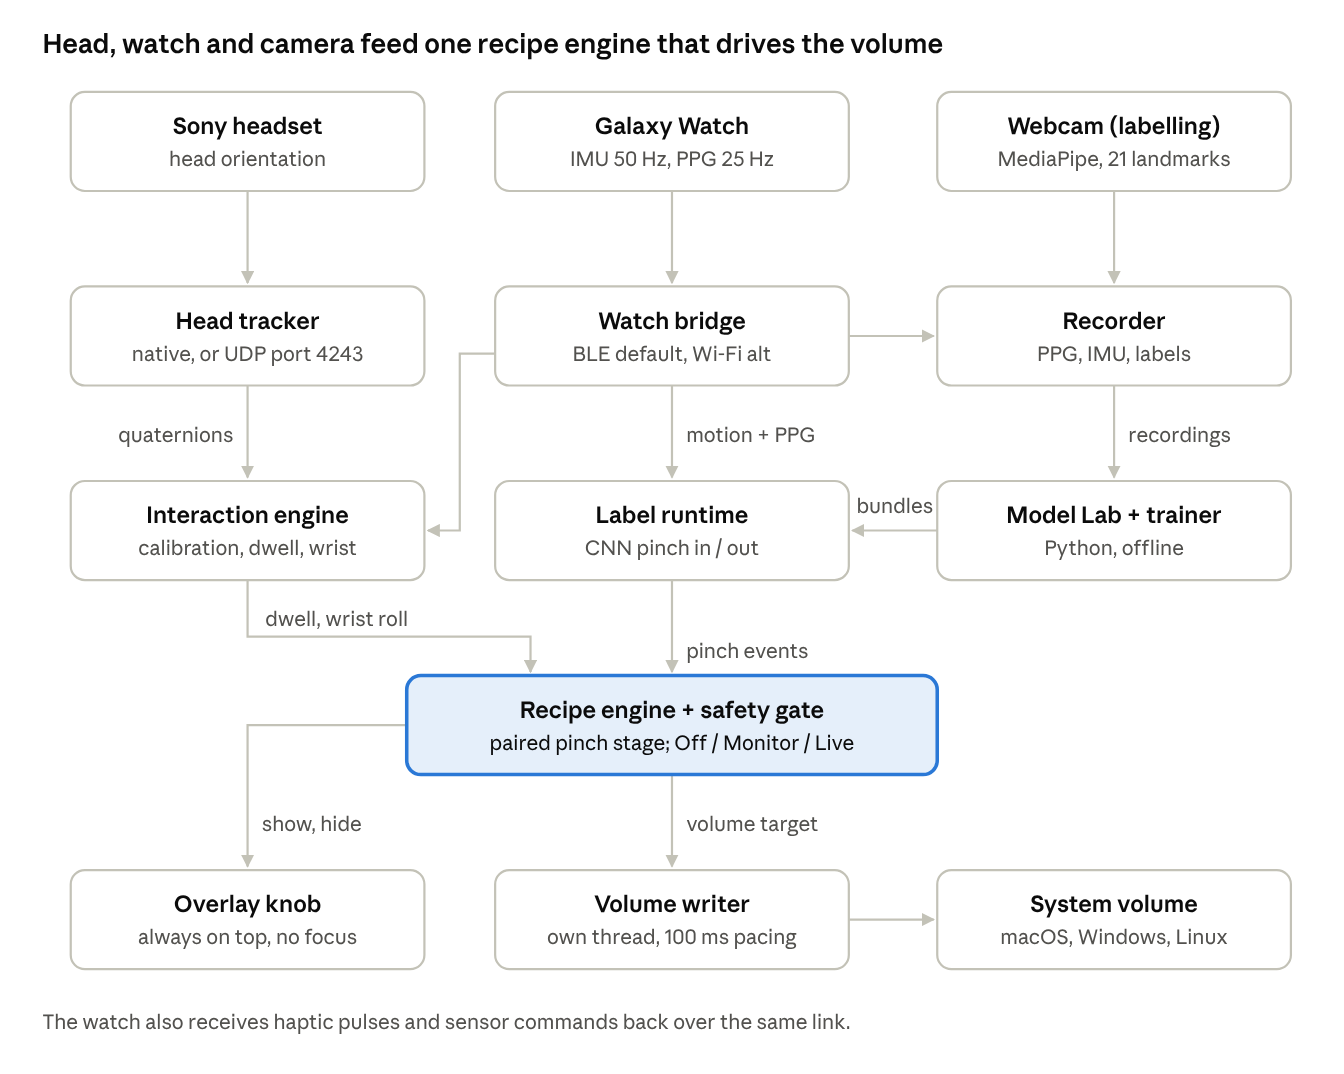
\includegraphics[width=0.82\textwidth]{architecture.png}
  \caption{System architecture. Head pose, wrist pose and pinch detections meet in one recipe engine, which alone may show the knob and drive the volume. The camera and trainer sit beside the live path and never act at runtime.}
  \label{fig:arch}
\end{figure*}

\begin{table}[t]
  \centering
  \caption{Devices and data rates}
  \label{tab:devices}
  \small
  \begin{tabular}{@{}lll@{}}
    \toprule
    Device & Data used & Rate \\
    \midrule
    Sony headset & Orientation quaternion & $\approx$25~Hz \\
    Galaxy Watch4+ & Rot.\ vector, lin.\ accel., gyro & 50~Hz \\
                   & Raw PPG green, red, IR & 25~Hz \\
                   & Crown button, wear state & On change \\
    Webcam & 21 hand landmarks (labels only) & 23--30~fps \\
    \bottomrule
  \end{tabular}
\end{table}

The target interaction has five steps. (1) The user looks at a calibrated location (top right by default) for a dwell time of 400~ms, and a transparent, non-focusable knob appears. (2) A \emph{pinch in} grabs the knob and records the wrist pose and current volume. (3) Wrist roll changes the volume relative to that pose. (4) A \emph{pinch out} releases the knob, keeping the volume, while the knob stays ready for another grab. (5) Looking away hides the knob; Escape cancels everything.

\subsection{Head Targeting}

During calibration the user faces the screen centre and then each named location, and the system stores a unit quaternion per target. At runtime the nearest target is found by angular distance,
\begin{equation}
  \theta = 2\arccos\bigl(\lvert q_{\mathrm{cur}} \cdot q_{\mathrm{tgt}} \rvert\bigr),
  \label{eq:angle}
\end{equation}
where the absolute value identifies $q$ and $-q$. A target activates when $\theta$ stays below an adjustable threshold for the dwell time. A change in the headset's reset counter means its reference frame moved and invalidates the calibration.

\subsection{Wrist-to-Volume Mapping}

At grab time the watch orientation $Q_s$ is stored, and each new sample yields
\begin{equation}
  Q_{\mathrm{rel}} = Q_s^{-1} Q_{\mathrm{cur}},
  \label{eq:qrel}
\end{equation}
from which the twist about the forearm axis is extracted. The volume target is absolute from the grab pose, so errors do not accumulate. The final mapping uses a 1$^\circ$ dead zone and about one volume point per 3$^\circ$, with a sensitivity setting and a direction switch. Table~\ref{tab:filters} lists the filters. Native volume calls on macOS take 130--190~ms, so a dedicated writer thread applies the newest target, keeping the sensor event loop free.

\begin{table}[t]
  \centering
  \caption{Volume filters and limits}
  \label{tab:filters}
  \small
  \begin{tabular}{@{}ll@{}}
    \toprule
    Stage & Rule \\
    \midrule
    Velocity outlier & Freeze target above max.\ angular velocity \\
    Jitter rejection & Accept target changes $\geq 0.5$ points \\
    Easing & Exponential, 150~ms time constant \\
    Slew limit & $\leq 30$ points/s, independent of input rate \\
    Write pacing & $\geq 100$~ms apart, writer thread \\
    Interaction epoch & Drop writes from a released grab \\
    Clamp & 0--100 \\
    \bottomrule
  \end{tabular}
\end{table}

\subsection{Watch Sensing Pipeline}

Both transports carry the same JSON envelopes (type, version, device id, sequence, timestamp and payload) and share one decoder. Over BLE the watch is a GATT peripheral and the desktop the central; the desktop assigns the device identity and requires both operating-system bonding and an explicit on-watch trust approval. Motion travels in 100~ms batches and PPG at each sensor flush (10~Hz by default), about 30 notifications per second.

Building this path exposed several faults (Table~\ref{tab:datapath}). Fragments sized as MTU$-3 = 514$~bytes exceeded the 512-byte attribute limit, so Android silently refused every PPG batch over BLE. An unbounded queue grew to seconds of delay when arm movement weakened the radio path, and was then discarded whole; it was replaced by a half-second queue that drops the oldest whole messages. Sending each motion reading separately produced about 61 notifications per second and saturated the link. After batching motion and PPG as separate streams, a 15-minute log showed 20 dropped messages (about 2~s of data), almost all just after reconnects. Timestamps stay on the watch's monotonic clock, while freshness and safety decisions use the desktop's own clock.

\begin{table}[t]
  \centering
  \caption{Measured properties of the watch data path}
  \label{tab:datapath}
  \small
  \begin{tabular}{@{}ll@{}}
    \toprule
    Quantity & Value \\
    \midrule
    Motion sensor rate & 49.8~Hz per sensor \\
    PPG rate & 25.0~Hz in every session \\
    PPG timestamp jitter & 6--10\% of gaps over 60~ms \\
    BLE MTU (Mac) & 517 (512~B per notification) \\
    Notifications/s & $\approx$61 before, $\approx$30 after \\
    Watch CPU at 61/s & App 21\%, BLE service 41\% \\
    Desktop CPU & App 10\%, web view 13\% \\
    Live inference & $\approx$0.2~ms/window (debug build) \\
    \bottomrule
  \end{tabular}
\end{table}

\subsection{Recipe Engine and Safety}

A recipe chains a head stage, a gesture stage and a wrist stage into an action on a virtual device, with conflict detection between recipes that would drive the same output. A pinch-in detection is a one-shot event, and detector silence is not a release. A \emph{paired} stage therefore latches the grab on a fresh pinch-in while the head target is held, ignores repeated starts while grabbed, releases on pinch-out (release wins if both arrive together) and cancels on head exit, Escape, data loss, model change or leaving live mode.

The effects are bounded by a fail-closed chain. An ordering watermark, a quality gate, a window-length check, a fusion freshness check (orientation older than 500~ms is rejected) and a gesture policy each force a release when they reject data. A watchdog releases any grab whose model data has been silent for 750~ms. Inference runs \emph{Off}, \emph{Monitor} (scores but never acts) or \emph{Live} (acts only through explicit intent bindings), and a saved Live setting is capped to Monitor at start-up. Model bundles are data-only, and their SHA-256 hash and input contract are re-verified on every load.

\section{Data Collection and Reference Annotations}\label{sec:data}

\subsection{Recordings}

All recordings were made by a single participant (the author), with the watch on the left wrist. Recordings are immutable bundles of PPG, motion and labels. Pinch is labelled as \texttt{pinch\_in} (contact), \texttt{pinch\_hold} and \texttt{pinch\_out} (release). Fist, thumbs-up and three kinds of everyday noise (typing, mouse use and ordinary activity) serve as negatives. Table~\ref{tab:data} summarises the collections used in this article.

\begin{table*}[t]
  \centering
  \caption{Collections used in this study (one participant, left wrist)}
  \label{tab:data}
  \small
  \begin{tabular}{@{}p{0.21\textwidth}p{0.43\textwidth}p{0.28\textwidth}@{}}
    \toprule
    Collection & Content & Used for \\
    \midrule
    September--October 2026 & 17 usable recordings; cue-based labels & Early PPG studies, training for the held-out test \\
    14 October 2026 & 15 recordings: 9 pinch, 4 fist, 2 everyday activity; strap refitted & One-shot held-out test; mixed-era study \\
    Frozen benchmark & 37 recordings, 1{,}390 events & IMU fusion and trigger studies \\
    October--November 2026 & Camera-timed pinch sessions, everyday noise & CNN versus trees, final models \\
    Leave-one-day-out set & 372 camera-marked pinches & Table~\ref{tab:lodo} \\
    Hand-labelled collection (Nov 2026) & 37 exports, 28 distinct sensor streams; manual label overrides & Hand-labelled development model (Table~\ref{tab:hand}) \\
    \bottomrule
  \end{tabular}
\end{table*}

\subsection{Camera Reference Annotations and Clock Alignment}

Early labels came from on-screen cues, and each recording had its own lag of up to 1.3~s between cue and execution. We therefore recorded camera reference annotations. MediaPipe~\cite{mediapipe} finds 21 hand landmarks per frame in the application's web view, without network access. Only landmarks are stored, never images. The watch and the browser keep different clocks. Watch timestamps are paired with browser arrival times every 200~ms, and since delivery delay is never negative, the smallest arrival-minus-watch difference estimates the offset.

Pinch contact is marked from the distance between thumb and index tips. A fixed threshold of 0.35 hand sizes missed many real pinches, because apparent distance depends on hand orientation. Those missed pinches were then trained as non-pinches and counted as false activations. Judging each session against its own hand reduced false activations on pinch sessions from 110 to 20 per hour. A later audit found 8 of 163 camera-labelled pinch-in intervals immediately followed by pinch-out with no hold, and queued them for review.

\section{Detection Methods}\label{sec:methods}

Each label has its own binary detector. Both families below answer the same question at every PPG sample: did the gesture just start? Table~\ref{tab:models} compares them.

\subsection{Engineered Features and Extremely Randomised Trees}

Each PPG sample is z-scored against the preceding 1, 2 and 4~s. Slope, curvature and jerk are computed causally, and 21 statistics are taken over the last 0.3, 0.6 and 1.3~s (1{,}701 features). The same statistics are computed for each motion axis, its magnitude and its change, plus movement relative to the preceding 3~s (1{,}032 features). An ensemble of 300 extremely randomised trees~\cite{geurts2006extra}, with at least 3 samples per leaf and 70\% of inputs per split, is trained on the moment 0.88~s after each start as positive, and on matched moments after other gestures, inside holds and in quiet time as negatives.

\subsection{Compact 1-D Convolutional Network}

Nine channels (accelerometer, gyroscope, PPG green, red and infrared) are resampled to a 50~Hz grid. At each decision, every channel $c$ is centred and scaled over the causal grid $G$ of the last 549 ticks (about 11~s) and the last 50 ticks $W$ (1~s) are kept:
\begin{gather}
  m_c = \operatorname{med}_{j\in G} x_{c,j}, \qquad s_c = 1.4826\,\operatorname{med}_{j\in G} \lvert x_{c,j} - m_c \rvert, \\
  u_{c,t} = \sigma\!\left(\operatorname{clip}\!\left(\frac{x_{c,t} - m_c}{s_c + \epsilon_c}, -500, 500\right)\right), \quad t \in W,
  \label{eq:norm}
\end{gather}
where the floor $\epsilon_c$ is 0.02 for accelerometer axes, 0.01 for gyroscope axes and $0.001(\lvert m_c\rvert + 1)$ for PPG. The 450 values $u_{c,t}$ are the input. Earlier models instead z-scored each tick against the 10~s before it (Section~\ref{sec:blind}). Three dilated convolutions (32, 32 and 64 channels, kernel 5, dilation 1, 2 and 4) with batch normalisation feed per-channel max and mean pooling, a 32-unit dense layer with dropout and a single output. Three networks trained with different seeds are averaged. Samples 0.4--0.6~s after a start are positives; samples with no start between 1.2~s before and 0.2~s after are negatives, with at most 40{,}000 negatives per network and positives weighted up to 20 times. Training uses Adam (learning rate 0.001, weight decay 0.0001), 12 epochs and batches of 256.

\begin{table}[t]
  \centering
  \caption{The two detector families}
  \label{tab:models}
  \small
  \begin{tabular}{@{}lll@{}}
    \toprule
     & Trees & CNN \\
    \midrule
    Input & 2{,}733 features & $9 \times 50$ raw values \\
    Model & 300 ExtraTrees & 3 dilated 1-D CNNs \\
    Training moments & $\approx$1{,}000--1{,}300 & Tens of thousands \\
    Decision delay & $\approx$0.88~s & $\approx$0.5~s \\
    History needed & 5.6~s & 11~s \\
    \bottomrule
  \end{tabular}
\end{table}

\subsection{Detection Rule and Threshold Selection}

After the score has reached the activation threshold, a detection is emitted causally at the first strictly decreasing score (the \emph{peak} trigger); its time is that decision, not a backdated maximum. It stays active until the score falls below the release threshold, 0.15 below activation, and the 1.5~s cooldown runs from that fall. The threshold is selected on training recordings only. Five models, each trained without one fifth of them, score the held-out parts in replay, and the threshold that catches the most starts within 30 false activations per hour is kept. The exported model is checked against the trained one before release. Shared fixtures keep the Python and Rust implementations of input building and detection identical.

\section{Evaluation Protocol}\label{sec:protocol}

Detectors are evaluated as continuous event detectors on complete recordings, and within each experiment training and test recordings are disjoint, with exported files of identical sensor data grouped as one source before splitting; one historical comparison row that reused training sessions is marked as such. Each emitted event is exactly one of: a \emph{catch} (inside the match window after a labelled start), a \emph{repeat} (another event during a caught gesture), \emph{late}, or a \emph{false activation}. The headline metrics are
\begin{gather}
  \mathrm{TAR} = \frac{\#\,\text{caught starts}}{\#\,\text{labelled starts}}, \label{eq:tar}\\
  \mathrm{FAR} = \frac{\#\,\text{false activations}}{\text{hours with no gesture under way}}. \label{eq:far}
\end{gather}
The FAR denominator is deliberately not the total recording time. Pinch sessions are dense, and a rate per hour of recording had hidden a model that fired about 175 times per hour of no-gesture time.

We used five study designs: recording-disjoint cross-validation judged first by worst-split (minimum) AUC; a one-shot held-out day with protocol and techniques frozen before the run; leave-one-day-out testing on camera-timed sessions with everyday noise; replays with real motion bursts spliced in before held-out pinches; and ablations of preprocessing, triggers and labels. Each study records whether its data had been seen before. Explored cross-validation is reported as progress evidence, not as an untouched test. Under a constant-rate Poisson assumption, zero false activations observed in $T$ hours bounds the rate at
\begin{equation}
  \lambda_{95\%} \approx \frac{-\ln 0.05}{T} \approx \frac{3}{T}\ \text{per hour},
  \label{eq:poisson}
\end{equation}
so 30 clean minutes still allow about six false activations per hour.

\section{Results}\label{sec:results}

\subsection{RQ1: PPG Alone}

A PPG ``step'' at pinch onset appeared in every early pinch session on all three channels, in units of each session's recent past. Its rest controls, however, had been chosen only by distance from gesture edges, and a recheck found 84\% of them (1{,}645 of 1{,}958) inside gestures, mostly in the middle of long holds. Against mid-hold moments the step separated well (median AUC 0.94). Against fist and thumbs-up starts it reached only about 0.65, needed about 700~ms after the start, and did not transfer between days (0.81 and 0.37 on two other days). As a continuous detector it found under 10\% of pinches at about one false activation per minute.

On a one-shot held-out day (14 October 2026: 208 pinch starts, 80 everyday-activity moments, 68 fist starts), every October PPG technique scored 0.60--0.64 AUC against non-pinch moments, with intervals reaching about 0.45. Fist starts were not separable from pinch starts (0.37--0.57), and no technique was usable continuously.

A mixed-era study then pooled 32 recordings (the 17 originals and the 15 refitted-strap recordings) in 20 recording-disjoint 60/40 splits. Raw-waveform neural networks were weak (mean AUC 0.47--0.58), and causal normalisation proved essential. Table~\ref{tab:mixed} shows that none of the robustness methods produced a clear gain in worst-split AUC over the base references. The reference PPG-only tree pipeline, over 37 recordings and 20 folds, reached minimum, mean and pooled event AUC of 0.7885, 0.8426 and 0.8105, with 41.15\% recall at 15.09 false activations per minute and about 830~ms latency. On recordings without any pinch it fired 19--25 times per minute. \emph{Answer to RQ1: on this watch, PPG carries a real but weak, slow and non-specific onset cue, and PPG alone does not support a continuous detector.}

\begin{table}[t]
  \centering
  \caption{Mixed-era robustness screen (AUC over 20 splits)}
  \label{tab:mixed}
  \small
  \begin{tabular}{@{}lrrr@{}}
    \toprule
    Method & Min & Mean & Max \\
    \midrule
    Reference A: RGB waveform, HGB & 0.676 & 0.749 & 0.842 \\
    Reference B: z-score, dense MLP & 0.661 & 0.756 & 0.853 \\
    Group DRO~\cite{sagawa2019dro} & 0.618 & 0.742 & 0.832 \\
    Causal morphology + HGB & 0.675 & 0.785 & 0.914 \\
    MiniRocket-like~\cite{dempster2020minirocket} & 0.653 & 0.745 & 0.851 \\
    Constrained derivative DTW & 0.682 & 0.739 & 0.816 \\
    Feature-space augmentation & 0.643 & 0.743 & 0.863 \\
    CORAL adaptation~\cite{sun2016coral} & 0.462 & 0.533 & 0.606 \\
    \bottomrule
  \end{tabular}
\end{table}

\subsection{RQ2: Inertial Fusion, Trigger Rule and Model Family}

On the frozen benchmark (37 recordings, 1{,}390 events, 20 splits), inertial features alone already outperformed PPG. Fused with PPG they raised worst-split AUC from 0.789 to 0.837, better on 19 of 20 splits. Separation of pinch from other gesture starts rose from 0.70 to 0.79--0.81. At a threshold of 0.5, false activations on recordings without a pinch fell from 19.0 to 12.0 per minute.

The original trigger fired at the first threshold crossing. At low thresholds this was often before the scoring window, and its 1.5~s lockout then blocked the correct firing. Firing at the peak of the score added 4--12 recall points at the same false-activation budget, at a cost of 35--90~ms of latency. Shifting labels earlier by 200--350~ms converted only about three false activations per minute into catches, so most remaining false activations were genuine responses to other movement.

Table~\ref{tab:lodo} reports historical leave-one-day-out results for the CNN on 372 camera-marked pinches. Pooled, the selected configuration caught 161 (43\%), with strong day-to-day variation: 21/171 and 37/52 on the two October days against 67/92 and 36/57 on the two November days. On the newer sessions the CNN caught about two thirds of pinches, against 10--28\% for the tree ensembles, and fired about 0.4~s sooner. A still-hand rule applied during training removed every moving moment, so the model never learned that movement is not a pinch. The best configuration trains without that rule and with everyday noise. The participant reports that pinch in and pinch out both work in the paired volume interaction. \emph{Answer to RQ2: inertial fusion and the peak trigger each improve detection substantially, and the compact CNN on raw channels outperforms engineered-feature trees on new sessions, but transfer across days varies widely.}

\begin{table*}[t]
  \centering
  \caption{CNN variants, leave one day out, 372 camera-marked pinches}
  \label{tab:lodo}
  \small
  \begin{tabular}{@{}lrrr@{}}
    \toprule
    Training & Caught & FAR noise (/h) & FAR pinch (/h) \\
    \midrule
    October only, no noise (earlier)$^\ast$ & 204 (55\%) & 143 & 23 \\
    With still-hand rule & 146 (39\%) & 23 & 20 \\
    \textbf{Without the rule, with noise} & \textbf{161 (43\%)} & \textbf{7} & 49$^\dagger$ \\
    Rule only at runtime & 130 (35\%) & 3 & 16 \\
    \bottomrule
  \end{tabular}\par\smallskip
  {\footnotesize FAR noise: false activations per hour on unseen everyday-noise sessions; FAR pinch: on pinch sessions.
  $^\ast$Trained on most October pinches, so not unseen. $^\dagger$Dominated by one day; other days 0--28/h.\par}
\end{table*}

\subsection{Hand-Labelled Development Model}\label{sec:hand}

Labels were later corrected by hand in the application's labelling view; a non-empty manual label overrides the original row label, and a blank one keeps it. The corrected collection has 37 exports, which reduce to 28 distinct sensor streams once identical exports are grouped. A median-scaled CNN trained on 20 of these recordings, with its 0.99 threshold chosen on training recordings only, was evaluated on eight others. Replaying the stored model (SHA-256 \texttt{ae0a22bf\ldots}) with the trainer's own detection and event-accounting code reproduced its stored metrics exactly (Table~\ref{tab:hand}). It caught 47 of 57 annotated pinch-in starts, 72--94\% by day, with four late detections, no repeats and no false activations over 0.48~h of eligible no-gesture time, and no interior input gaps. Median latency from annotated start to causal detection was 442~ms. The everyday-activity session's highest score was 0.970 against the 0.99 threshold, so the zero false-activation result rests on a narrow margin. These are development results for one participant and one target; the evaluation recordings are not established as untouched by development.

\begin{table}[t]
  \centering
  \caption{Hand-labelled pinch-in model, replay on its eight evaluation recordings}
  \label{tab:hand}
  \small
  \begin{tabular}{@{}ll@{}}
    \toprule
    Measure & Value \\
    \midrule
    Caught & 47/57 (82.5\%) \\
    Missed & 10 (4 late, 6 undetected) \\
    Repeats, false activations & 0, 0 \\
    No-gesture time & 0.48~h \\
    95\% upper bound, false act. & 6.2/h \\
    Latency, median (IQR) & 442 (384--510)~ms \\
    \bottomrule
  \end{tabular}
\end{table}

\subsection{A Normalisation Blind Spot}\label{sec:blind}

The first CNN normalised each channel by a rolling 10~s mean and standard deviation. A burst of wrist motion raised the gyroscope deviation from about 0.03 to about 1~rad/s, shrinking a following pinch roughly thirty-fold until the burst left the window. No training pinch had experienced this: the largest 1~s gyroscope RMS before any of 459 pinch starts was 0.62~rad/s, whereas everyday noise reached 14~rad/s. A window-score diagnostic (Table~\ref{tab:hangover}) spliced real bursts into held-out recordings and counted a pinch if the peak score 0.1--1~s after its start reached the threshold. It is not a continuous event replay or a live test, but it shows that the median/MAD scaling of (\ref{eq:norm}) removes the blind spot for bursts up to about 4~s; motion lasting 6~s or more still causes a 3--6~s blackout.

\begin{table}[t]
  \centering
  \caption{Window-score diagnostic after a spliced motion burst (ends 1~s before the pinch)}
  \label{tab:hangover}
  \small
  \begin{tabular}{@{}lrrrr@{}}
    \toprule
     & \multicolumn{2}{c}{Pinch in} & \multicolumn{2}{c}{Pinch out} \\
    Burst & Roll. & Med. & Roll. & Med. \\
    \midrule
    None & 92\% & 92\% & 98\% & 98\% \\
    3--6~rad/s, 2~s & 0\% & 93\% & 5\% & 98\% \\
    2.5--6~rad/s, 4~s & 0\% & 87\% & 4\% & 89\% \\
    2--6~rad/s, 6~s & 0\% & 58\% & 6\% & 28\% \\
    2--6~rad/s, 8~s & 0\% & 16\% & 0\% & 4\% \\
    \bottomrule
  \end{tabular}
\end{table}

\subsection{Further Variations}

Table~\ref{tab:variations} summarises the variations that were tried and rejected or deferred. A three-stage curriculum (newest clean sessions, then older camera-labelled sessions, then noise) reached 78.9\% recall for pinch-in (15/19, median latency 469~ms) and 52.6\% for pinch-out (10/19, 390~ms) at zero false activations on a reserved validation pair. Training on the newest clean data plus noise alone did not transfer to older sessions (4.9--31.4\% recall). Because the same pair chose the threshold and supplied the metric, and it contains only 19 starts, this is validation evidence only.

\begin{table*}[t]
  \centering
  \caption{Variations tried}
  \label{tab:variations}
  \small
  \begin{tabular}{@{}p{0.25\textwidth}p{0.47\textwidth}p{0.2\textwidth}@{}}
    \toprule
    Variation & Result & Decision \\
    \midrule
    Retrain on own false alarms & Recall 27\% vs 31\%, no fewer false activations & Off \\
    2~s window, fourth convolution & 49--51\% vs 45\% at $\approx$20/h; chosen threshold exceeded budget on noise & Deferred \\
    Self-supervised pretraining & 27 vs 7 false activations/h on noise; 152 vs 168 catches at equal FAR & Rejected \\
    Still-hand rule in training & Model never learns that movement is not a pinch & Off for CNN \\
    Fixed camera-mark threshold & 110 false activations/h on pinch sessions & Per-session marks (20/h) \\
    Pinch-shape and Haar-wavelet features & No gain for PPG + IMU; wavelet detail did not set a pinch apart & Not adopted \\
    \bottomrule
  \end{tabular}
\end{table*}

\subsection{Double-Pinch Gating}

For a double-pinch gesture we specified an envelope of data preconditions and context gates, outside which the detector abstains, followed by candidate checks before any model score counts. On 278 camera-timed contacts, gates and checks kept about 80\% of single pinches. They cut candidate jolts from 76 to 0.6 per minute during arm movement and from 40 to 0.4 during wrist twists. These thresholds are starting values to be re-measured at 100~Hz.

\subsection{System Performance}

Every optimisation was measured before it was made, on an Apple M3 laptop. Appending to the full dataset buffer fell from 452~$\mu$s to 0.1~$\mu$s, and the old path had also corrupted row order beyond 200{,}000 rows. Repeated raw-signal viewer requests fell from a full 52~ms re-parse to 1.3~$\mu$s from a bounded cache. Status events at orientation rate fell from up to 200 to about 10 per second. Processing a long recording in the trainer fell from 7.26 to 2.23~s, and the release binary shrank from 17.5 to 12.0~MB. Live inference costs about 0.2~ms per window in a debug build.

\section{Discussion}\label{sec:discussion}

\subsection{RQ3: What Made Offline Results Predictive}

The largest errors in this project came from evaluation rather than from code. Four practices inflated results before they were corrected: rest controls that were really mid-gesture, explored recordings reused as tests, false-activation rates over the wrong denominator, and per-window AUC used as if it were a release metric. Two labelling practices mattered as much as any model change. Cue-based labels carried a per-recording lag of up to 1.3~s, and a fixed camera threshold silently turned real pinches into negatives. Training-time filters also change what a model learns: the still-hand rule, meant to reduce false activations, prevented the model from learning that movement is not a pinch. \emph{Answer to RQ3: offline results became predictive only once evaluation replayed whole recordings through the deployed trigger, counted false activations per hour of no-gesture time, protected test sets from exploration and used camera-timed, per-session labels.}

\subsection{Implications}

For stock smartwatches, inertial sensing should be treated as the primary pinch signal, with PPG as a complementary channel. This agrees with OpenWatch's finding that PPG adds to inertial data rather than replacing it~\cite{bonazzi2026openwatch}. Small raw-signal networks with robust normalisation and everyday negatives generalise better than large engineered feature sets. Finally, the interaction design matters. Gating gestures on gaze dwell and requiring a paired release make occasional false detections far less costly than in an always-armed detector.

\subsection{Threats to Validity}

\textbf{Internal validity.} Thresholds were chosen on training data only, but most collections were explored during development; only the 14 October test was a true one-shot test. The hand-labelled model's evaluation recordings were listed separately from its training set, but whether they informed labelling or model selection was not recorded, its training configuration had to be reconstructed for the replay, and its zero false-activation result rests on a 0.02 margin below the threshold. No hand-labelled pinch-out model exists yet. Camera labels depend on landmark accuracy and clock alignment, whose residual error was not independently measured.

\textbf{External validity.} All data come from one participant, one watch and one wrist, mostly at 50~Hz motion; pinches made while moving are rare. Results may not transfer to other people, devices or activities.

\textbf{Construct validity.} False activations were measured on recorded everyday-noise sessions rather than on full days of natural use, so the hourly rates are estimates over limited exposure (see (\ref{eq:poisson})).

\section{Limitations and Future Work}\label{sec:future}

Sessions recorded on 14 October remain poorly detected (12--18\%) by every model trained on other days, against 63--75\% on 3--4 November. The next step is a sealed test, collected after freezing the model, preprocessing, thresholds and protocol. It should span several days with strap refits, and include 30--60 minutes of continuous everyday activity per session and pinches made while moving, recorded at 100~Hz. Per-user or per-session adaptation, which raised ViWatch from 45\% to 97\%~\cite{viwatch2023}, is the most promising modelling direction. A 2~s input window with stricter threshold selection is a second candidate. On the engineering side, open items are Wi-Fi peer authentication, physical validation on Windows and Linux, signed packaging and a BLE battery trial. The same look-pinch-turn interaction can then be extended to brightness and scrolling.

\section{Conclusion}\label{sec:conclusion}

A consumer headset and smartwatch can control a laptop through a look-pinch-turn interaction. Head orientation selects the control, a compact CNN on watch motion and PPG detects pinch in and pinch out, and wrist roll sets the value, all behind a fail-closed safety chain. Wrist PPG alone was not sufficient on a stock watch. Inertial fusion, camera-timed labels and event-based evaluation were what turned the detector from a promising offline score into a working interaction.


\backmatter

\bmhead{Acknowledgements}
[Acknowledgements, or remove this heading.]

\section*{Declarations}

\begin{itemize}
\item \textbf{Funding:} [State funding sources, or ``Not applicable''.]
\item \textbf{Conflict of interest/Competing interests:} The author declares no competing interests. [Confirm, and use the heading the journal requires.]
\item \textbf{Ethics approval and consent to participate:} All recordings were made with the author as the only participant; no other people took part. [Confirm whether an ethics approval or waiver is required for self-recorded physiological data, and state it.]
\item \textbf{Consent for publication:} [Not applicable, or state.]
\item \textbf{Data availability:} [State where the recordings can be obtained, or ``available from the author on reasonable request''.]
\item \textbf{Materials availability:} [Not applicable, or state.]
\item \textbf{Code availability:} [State the repository URL and licence, or the access conditions.]
\item \textbf{Author contribution:} V.B. designed and built the system, collected and analysed the data, and wrote the manuscript. [Confirm.]
\end{itemize}

\bibliography{refs}

\end{document}
